\chapter{Experiments} \label{chapterexperiments}
In this chapter we introduce experiments and their results for our implementation of all algorithms described in the previous chapter.
In order to test the performance of algorithms we have implemented data set generator providing artificial data sets with various properties.

\section{Data set generator}
When we want to generate $n$ observations without outliers that satisfies linear regression model we can do it as follows:

\begin{algo}[Generate clean data] \label{generate:linear:model}
    \mbox{}\vspace{\dimexpr-\baselineskip-\topsep}
\\
    \begin{enumerate}
        \item Generate regression coefficients $\vec{w} = (w_1, \ldots, w_p)$ at random and set a possible $\sigma^{2}$.
        \item Generate random explanatory variables $\vec{x_i}$.
        \item Generate random noise $\varepsilon_i \sim \mathcal{N}(0,\,\sigma^{2})$.
        \item Compute dependent variable $y_i = \vec{w}^T\vec{x_i} + \varepsilon_i$.
        \item Repeat steps $2$--$4$ $n$ times.
    \end{enumerate}
\end{algo}
As a result we obtain a data set stored in the matrix $\vec{X}$ and vector $\vec{y}$. Regression coefficients can be set to arbitrary values. All $\vec{x_i}$ should be generated independently but to avoid huge numbers we generate all $\vec{x_i}$ from some normal distribution. 

Another thing that needs to be considered is the intercept. In this work we assumed that our data already include intercept, so in that case $w_1$ is equal to intercept and all $x_{i1}$ should be equal to $1$. Note that the same result can be obtained by generating data without intercept and with $\varepsilon_i \sim \mathcal{N}(\mu,\,\sigma^{2})$ for some $\mu \in \mathbb{R}$. We can then extend matrix $\vec{X}$ by adding the first column that contains only $1$s. This approach is very common and software for estimating regression coefficients usually allows to set parameter which determines if intercept should be used; if so, the column of $1$s is added. For that reason we generate our data sets using this approach. That means we generate $\varepsilon_i \sim \mathcal{N}(\mu,\,\sigma^{2})$ and column of $1$s is included only in case we set parameter for using intercept when fitting the data set. 

\subsection{Generating outliers}
As we have already described in Section~\ref{outliers:info}, we distinguish different types of the outliers: vertical outliers and two types of leverage points --- good leverage points and bad leverage points. Those types of outliers are visualized in Figure~\ref{outliers:types:figure}. We can see that good leverage points are not deemed as an outliers here, even if they are distant observations, because they follow the linear pattern. 

\begin{figure}[h]
    \centering
    
% even more fun
\begin{tikzpicture}
    \begin{axis}[
        xlabel={$\vec{x}$},
        ylabel={$y$},
        xmin=0,
        xmax=5,
        ymin=0,
        ymax=7,
        xtick = {0},
        ytick = {0}, 
        domain = 0:8,
        axis lines = middle,
        clip=false
      ]
    
      % VERTICAL OUTLIERS
      \addplot[soldot, red]coordinates {(1.25,5.25*0.8+0.85)} node [anchor=north west,text=black] {Vertical outliers};
      \addplot[soldot, red]coordinates {(1.2,5.4*0.8+0.95)} node [anchor=north east,text=black] {};
      \addplot[soldot, red]coordinates {(1.35,5.4*0.8+1.1)} node [anchor=north east,text=black] {};


      % REGULAR OBSERVATIONS
      \addplot[soldot,black]coordinates {(2.45, 2.45*0.8+0.94)} node [anchor=north east,text=black] {};
      \addplot[soldot,black]coordinates {(2.2, 2.3*0.8+1.12)} node [anchor=north east,text=black] {};
      \addplot[soldot,black]coordinates {(2.1, 2.1*0.8+0.8)} node [anchor=north west,text=black] {Regular observations};
      \addplot[soldot,black]coordinates {(2, 2*0.8+1.1)} node [anchor=north east,text=black] {};
      \addplot[soldot, black]coordinates {(1.7,1.7*0.8+1)} node [anchor=north east,text=black] {};
      \addplot[soldot, black]coordinates {(1.5,2.295)} node [anchor=north east,text=black] {};
      \addplot[soldot,black]coordinates {(0.8, 0.8*0.8+1.1)} node [anchor=north east,text=black] {};
      \addplot[soldot, black]coordinates {(1.25,1.25*0.8+0.8)} node [anchor=north east,text=black] {};
      \addplot[soldot, black]coordinates {(1.2,2.28)} node [anchor=north east,text=black] {};
      \addplot[soldot, black]coordinates {(0.6,1.4)} node [anchor=north east,text=black] {};
      \addplot[soldot, black]coordinates {(0.9,1.8)} node [anchor=north east,text=black] {};
      
      % GOOD LEVERAGE POINTS
      \addplot[soldot,black]coordinates {(5, 5*0.8+0.94)} node [anchor=north east,text=black] {};
      \addplot[soldot,black]coordinates {(4.8, 4.8*0.8+1.1)} node [anchor=north west,text=black] {Good leverage points};

      % BAD LEVERAGE POINTS
      \addplot[soldot,red]coordinates {(5.51, 0.5)} node [anchor=north east,text=black] {};
      \addplot[soldot,red]coordinates {(5.7, 0.6)} node [anchor=north west,text=black] {Bad leverage points};

      % plot of main model
      \addplot [domain=-1:6, samples=2, dashed] {0.8*x+1};      
    \end{axis} 
\end{tikzpicture}

    \caption{Different types of outliers.  }
    \label{outliers:types:figure}
\end{figure}

Moreover, the data set can contain multiple observations that satisfies linear regression model but with different regression coefficients. That means such data set can contain data from multiple different models.

To generate the vertical outliers we only need to modify step $3$ of Algorithm~\ref{generate:linear:model}. We have multiple options:
\begin{itemize}
    \item Generate $\varepsilon_i$ from $\mathcal{N}(\mu,\,\sigma^{2})$ but use different parameter  $\mu$ and $\sigma^{2}$.
    \item Generate $\varepsilon_i$ from some heavy tailed or asymmetrical distribution like  Log-normal or exponential distribution.
    \item Combine both above so that we randomly choose distribution and randomly generate parameters for such distribution.
\end{itemize}
The last option is the most versatile so we use it in our data generator.

Because we generate $\vec{x_i}$ from the normal distribution, we can generate leverage points just by changing parameter $\mu$  of this distribution. If we consequently generate $\varepsilon_i$ from the same distribution with the same parameters as for the regular observations, we obtain good leverage points. On the other hand if we generate $\varepsilon_i$ as described above, we obtain bad leverage points.

If we want to generate outliers that correspond to the different model we can just choose the regression coefficients $\vec{w}$ differently. It is also possible to use different parameters of normal distribution for generating $\vec{x_i}$ and parameters for generating $\varepsilon_i$. Theoretically, we are able to introduce outliers even into this model, but when this model is an ``outlier'' by itself relative to the original model, it is not needed. By this approach are able to generate the observations from arbitrary number of different models, but for the sake of the simplicity we use only one different model in our data sets.

\section{Data sets}
We have implemented random data set generator as described in the previous section with the following parameters:
\begin{itemize}
    \item $n$ and $p$ for setting the number of the generated observations and the dimension of the explanatory variables,
    \item $outlier\_ratio$ for setting proportion of the outliers in the data set. This include vertical outliers, bad leverage points and also outliers from the second model,
    \item $leverage\_ratio$ is proportion of the explanatory variables that are generated as leverage points,
    \item $\mu_{\vec{x}}, \sigma^{2}_{\vec{x}}$ are the parameters of the normal distribution for generating non outlying $\vec{x_i}$,
    \item $\mu_{\vec{x_o}}, \sigma^{2}_{\vec{x_o}}$ are the parameters of the normal distribution for generating outlying $\vec{x_i}$ (leverage points),
    \item $\mu_{\varepsilon}, \sigma^{2}_{\varepsilon}$ are the parameters of the normal distribution for generating non outlying errors $\varepsilon_i$,
    \item $\mu_{\varepsilon_o}, \sigma^{2}_{\varepsilon_o}$ are the parameters of the distribution for generating outlying errors $\varepsilon_i$,
    \item $distrib_{\varepsilon_o}$ is the distribution from which outlying errors are generated --- options are normal distribution, log-normal distribution and exponential distribution (when exponential distribution is chosen, then only $\sigma^{2}_{\varepsilon_o}$ parameter is used),
    \item $2m\_ratio$ is the proportion from the outliers which are generated from the second model,
    \item $\mu_{\vec{x_{M2}}}, \sigma^{2}_{\vec{x_{M2}}}$ and $\mu_{\varepsilon_{M2}}, \sigma^{2}_{\varepsilon_{M2}}$ are the parameters for normal distributions for generating $\vec{x_i}$ and $\varepsilon_i$, respectively, from the second model.
\end{itemize}

We used this generator to generate three data sets $D1$, $D2$ and $D3$ which differ by the types of the outliers they contain:
\begin{itemize}
    \item $D1$ contains outliers which are not from the second model: vertical outliers, bad leverage points and good leverage points ($2m\_ratio = 0$)
    \item $D2$ contains only outliers from the second model ($2m\_ratio = 1$),
    \item $D3$ contain outliers of all described types. ($2m\_ratio = 0.4$).
\end{itemize}

All three data sets are set to contain $20\%$ leverage points ($leverage\_ratio = 0.2$) and non outlying $\vec{x_i}$ are generated from $\mathcal{N}(0,10)$ (thus $\mu_{\vec{x}} = 0, \sigma^{2}_{\vec{x}} = 10$). Other parameters are independently randomly generated from uniform distribution so that:
\begin{itemize}
    \item $\mu_{\vec{x_o}} \sim \mathcal{U}(20,\,60), \sigma^{2}_{\vec{x_o}} \sim \mathcal{U}(10,\,20)$,
    \item $\mu_{\varepsilon} \sim \mathcal{U}(0,\,10), \sigma^{2}_{\varepsilon}  \sim \mathcal{U}(1,\,5)$,
    \item $\mu_{\varepsilon_o} \sim \mathcal{U}(-50,\,50), \sigma^{2}_{\varepsilon_o} \sim \mathcal{U}(50,\,200)$,
    \item $\mu_{\vec{x_{M2}}} \sim \mathcal{U}(-30,\,30), \sigma^{2}_{\vec{x_{M2}}} \sim \mathcal{U}(10,\,20)$,
    \item  $\mu_{\varepsilon_{M2}}  \sim \mathcal{U}(-10,\,10) , \sigma^{2}_{\varepsilon_{M2}}\sim \mathcal{U}(1,\,5)$,
    \item $distrib_{\varepsilon_o}$ is uniformly randomly set to normal, log-normal  or exponential distribution 
\end{itemize}
Finally, parameters $n$, $p$ and $outlier\_ratio$  are set separately for each particular experiment. Implemented data generator provides not only matrix $\vec{X}$ and vector $\vec{y}$ but also their subsets which does not contain outliers. This is useful, because it gives us the ability to compare appropriative solution to the original model.

\section{Implementation of the algorithms}
We have implemented all described algorithms, moreover, because algorithms for computing the feasible solution could be implemented both by calculating inversion and by calculating QR decomposition, we have implemented both version of those algorithms. Here is the list of all the implemented algorithm with their acronyms we use for labeling them:

\begin{description}
    \item[FAST-LTS] (Section~\ref{section_fast_lts} with all described improvements),
    \item[FSA-I] (Section~\ref{section_feasible_solution}),
    \item[FSA-QR] (FSA using theory from Section~\ref{oeamoeammea}),
    \item[MOEA-I] (Section~\ref{oeamoeammea} it is the improved version of OEA),
    \item[MOEA-QR] (MOEA using theory from Section~\ref{differentcomputation}),
    \item[MMEA-I] (Section~\ref{mmeasection}),
    \item[MMEA-QR] (MMEA using theory from Section~\ref{differentcomputation}),
    \item[BAB] (Section~\ref{sectionbab}),
    \item[BSA] (the implementation of improved BAB (BSABAB) from Section~\ref{bsasection}),
    \item[FAST-LTS-MMEA-I] (combination of algorithms from Section~\ref{sectioncombined}),
    \item[FAST-LTS-MOEA-I] (other combination of algorithm from Section~\ref{sectioncombined}),
    \item[FSA-QR-BAB] (BAB with sorting speedup as described in Section~\ref{sectionbab}),
    \item[FSA-QR-BSA] (BSABAB using our idea from Section~\ref{bsasection}),
    \item[RBSA] (probabilistic BSA using our idea from Section~\ref{bsasection}),
    \item[RANDOM] (random resampling algorithm outlined in section Section~\ref{first:attempts}).
\end{description}

These algorithms were first implemented in Python using the NumPy package~\cite{numpy}. To seed up the algorithms,we have implemented all the algorithms in \CC \ using the Eigen library~\cite{eigenweb} for matrix manipulation. Since it is very popular today to use Python for data processing and manipulation, we have used pybind11 library~\cite{pybind11}, that exposes \CC \ types for Python and vice versa and written Python wrappers around the \CC \ implementation. 

Moreover pybind11 allows to bind Eigen types directly to the NumPy types (because both libraries are LAPACK compatible), so that it is possible to share pointers to the matrices between Eigen and NumPy and hence the data does not have to be copied when transferring between Python an \CC.

Therefore the data generator, all tests and experiments are implemented in Python; the \CC \  code is called only within the Python wrappers. It is also appropriate to mention that the interface of the algorithms was created with regards to the popular scikit-learn package~\cite{scikit-learn}; the interface is almost identical, so all of the classes implementing the algorithms can be used in the same manner as classes from the scikit-learn linear regression module.


\section{Results}
In the two previous sections we have described our experimental setup. Here we report the results of our experiments.

\subsection{The strong necessary condition algorithms} \label{strong:experiments}
Here we present the results of multiple simulations where we compared speed and accuracy of the algorithm finding subsets satisfying the strong necessary condition. For each combination of parameters $n$, $p$ and $outlier\_ratio$ ($out$) we generated data sets  $D1$, $D2$ and $D3$ $100$ times (each time new data sets were generated) and run all algorithms on those data sets. Value of $h$ was conservatively chosen so that $h = [(n/2] + [(p+1)/2]$. For all the runs we used the intercept, hence the value of $p$ represents the dimension of $\vec{x}$ including intercept. All algorithms were set to run at most for $50$ steps and each of them is starting from $1$ randomly selected $h$-element subset.
\footnote{This was done primarily because the computation was exhaustive due to the large number of parameter combinations. In experiments we describe later, number of the starting subsets is higher.}
The results are given in Appendix~\ref{apendix:chapter} in Tables~\ref{table1}, \ref{table2} and \ref{table3} for data sets $D1$, $D2$ and $D3$, respectively. Beside CPU time, we also measured the cosine similarity and $L^2$ norm of the resulting estimate and the regression coefficients given by the original model which does not contain outliers. For $n > 500$, cells for the FSA-I and FSA-QR are empty, these algorithms were too slow and it would take weeks to finish all simulations.
In Figure~\ref{all_distances} are given box plots showing cosine similarity and $L^2$ norms of the results. 

As expected, the algorithms using the QR decomposition provide slightly better results. Moreover, the best results are given by the FSA-QR. On the other hand, both FSA-I and FSA-QR are much slower because they does not use bounding condition as in the case of MOEA-I and MOEA-QR. We can also see that MMEA-QR provides very similar results to the MOEA-QR. So in the case of algorithms finding strong necessary condition we would recommend using the FSA-QR for small data sets and for large ones the MMEA-QR. 

\begin{figure}[h]
    \centering
    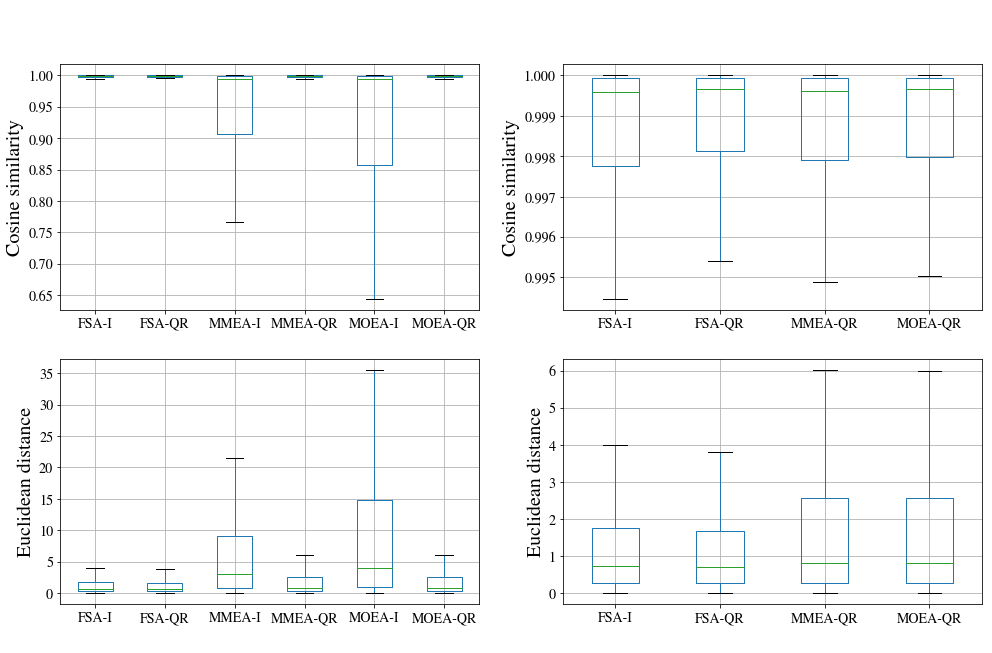
\includegraphics[width=14cm]{img/all_distances_feasible}

    \caption{Similarity of the solutions given by the algorithms finding $h$-element subsets satisfying strong necessary condition compared to the OLS solution on the subset of the data set that does not contain outliers. On the left are two box plots for all algorithms. Since the visualization is influenced by the scale of MMEA-I and MOEA-I box plots, we provide also two graphs without these two algorithms on the right.}
    \label{all_distances}
\end{figure}

\subsection{Algorithms for finding the exact solution}
Here we provide results of the algorithms finding the exact solution. For the improved versions of the BAB and BSA algorithms, which are able to incorporate pre-computed results, we decided to use the estimate given by the FSA-QR. This algorithm, as observed in previous section, provides the best results. FSA-QR is quite slow compared to the MOEA and MMEA variations, but because the exact algorithms have much higher time complexity (thus can be used only on very small data sets), this slowing down is insignificant with respect to the total time complexity.

The setup for the simulations was the same as in the previous section, but we only compare speed this time because all of the algorithms provide the exact solution. 

The results are given in Appendix~\ref{apendix:chapter} in Tables~\ref{table:exact:1}, \ref{table:exact:2} and \ref{table:exact:3} for data sets $D1$, $D2$ and $D3$ respectively. 
    
Interesting observation is given by the Figure~\ref{exact:improvement} depicting where is the average time of the calculation improved by the FSA-QR-BAB instead of the BAB and the FSA-QR-BSA instead of the BSA. Whereas FSA-QR-BAB improves the time of the computation significantly, the FSA-QR-BSA does not leads to any time improvement at all.
 
\begin{figure}[h]
    \centering
    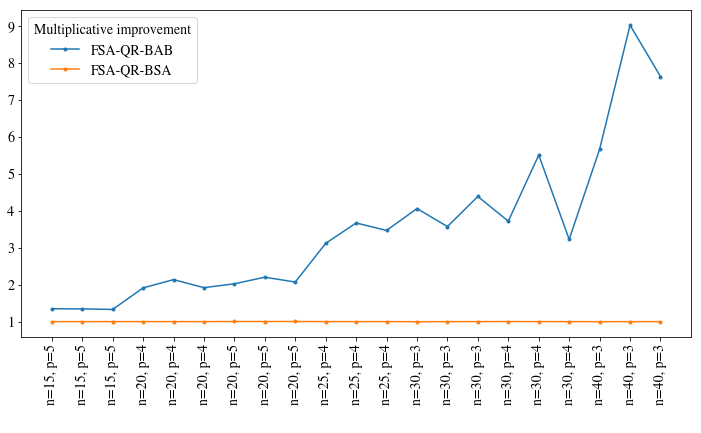
\includegraphics[width=12cm]{img/exact_improvement}

    \caption{For various combinations of parameters $n$ and $p$ we calculated average multiplicative improvement of the CPU time for running FSA-QR-BAB and FSA-QR-BSA instead of BAB and BSA.}
    \label{exact:improvement}

    
\end{figure}

We can observe from the results that BSA (as well as FSA-QR-BSA) is, as expected, sensitive to increasing the parameter $p$. On the other hand, when $p$ stays low, BSA outperforms both BAB and FSA-QR-BAB. We have ran $10$ simulations for higher values of $n$ for each dataset $D1$, $D2$ and $D3$ for algorithm BSA, while preserving value of $p = 2$. In this simulation we have not used intercept. Resulting average, minimum and maximum CPU times are given in Table~\ref{bsa:big:table}. For the data sets $D2$ and $D3$ the simulation was not performed for $n = 400$, so the 
respective cells are empty.


\begin{table}[h!]
    \centering

\scalebox{0.63}{
\begin{tabular}{l|l|l|r|r|r|r|r|r|r|r|r|} 
\hline\hline
&      & out & 
\multicolumn{3}{l|}{$D1$} &
\multicolumn{3}{l|}{$D2$} &
\multicolumn{3}{l|}{$D3$} \\  
\hline
$n$ & $out$ & $h$ &     avg &       min &       max &      avg &      min &      max &      avg &      min &      max \\
\hline
      100 & 0.10 & 51  &     5.499 &     5.213 &     6.860 &    5.206 &    5.150 &    5.273 &    5.215 &    5.166 &    5.342 \\    & 0.30 & 51  &     5.598 &     5.125 &     6.852 &    5.345 &    5.129 &    6.707 &    5.198 &    5.142 &    5.309 \\    & 0.45 & 51  &     5.978 &     5.161 &     6.902 &    5.347 &    5.099 &    6.724 &    5.425 &    5.164 &    6.989 \\200 & 0.10 & 101 &    81.172 &    80.042 &    81.582 &   81.280 &   80.816 &   81.575 &   82.678 &   81.153 &   93.849 \\    & 0.30 & 101 &    80.992 &    80.416 &    81.396 &   82.482 &   80.789 &   94.172 &   81.250 &   80.008 &   81.921 \\    & 0.45 & 101 &    81.101 &    80.660 &    82.054 &   81.165 &   80.836 &   81.496 &   81.332 &   81.088 &   81.631 \\300 & 0.10 & 151 &   422.982 &   421.551 &   423.973 &  425.611 &  422.521 &  466.379 &  423.312 &  422.593 &  424.112 \\    & 0.30 & 151 &   426.895 &   421.704 &   465.063 &  423.236 &  421.937 &  424.155 &  427.746 &  422.930 &  466.564 \\    & 0.45 & 151 &   427.169 &   421.060 &   467.341 &  427.391 &  421.636 &  466.195 &  423.404 &  422.699 &  424.172 \\400 & 0.10 & 201 &  1390.836 &  1378.586 &  1483.780 &      $-$ &      $-$ &      $-$ &      $-$ &      $-$ &      $-$ \\    & 0.30 & 201 &  1389.465 &  1373.600 &  1483.066 &      $-$ &      $-$ &      $-$ &      $-$ &      $-$ &      $-$ \\    & 0.45 & 201 &  1380.151 &  1373.839 &  1383.228 &      $-$ &      $-$ &      $-$ &      $-$ &      $-$ &      $-$ \\
\hline
\end{tabular}
% end table
}

\caption{Average, minimum and maximum CPU times of computation time for BSA for $p=2$ and various combinations of parameters $n$ and $out$  for each dataset.}
\label{bsa:big:table}

\end{table}


\subsection{FAST-LTS and combinations of the algorithms} \label{results:combinations}
In this section we present the results of the FAST-LTS algorithm compared to the MOEA-QR and MMEA-QR because, as described in Section~\ref{strong:experiments}, these algorithms seems to be very fast while providing reliable results. We also run simulations on the combinations of those two algorithms as described in Section~\ref{sectioncombined}. All algorithms were set to start from $50$ randomly chosen subsets for each simulation and maximum number of inner cycles was set to $40$. We ran simulations $100$ times for each combination of the parameters $n$, $p$ and $out$ for each data set. The results are given in Appendix~\ref{apendix:chapter} in Tables~\ref{table:combined:1}, \ref{table:combined:2} and \ref{table:combined:3} for data sets $D1$, $D2$ and $D3$ respectively. Beside measuring the cosine similarity and $L^2$ norm, we also provide the number of the inner cycles for each algorithms. We can see, that providing solution from the FAST-LTS to the MOEA-QR and MMEA-QR significantly reduce those numbers.
 
In Table~\ref{table:percentage:improvement} we can see that approximately in 30 $\%$ of cases MOEA-QR and MMEA-QR were able to improve the solution of the FAST-LTS in all three data sets. That means in those cases FAST-LTS algorithm have provided solutions that satisfied weak necessary condition but not the strong one. 

\begin{table}[h!]
    \centering
    \begin{tabular}{l|r|r|r|}
        \hline\hline
         &    $D1$ &    $D2$ &    $D3$ \\
         \hline
         FAST-LTS-MMEA-QR &  30.33 $\%$ &  34.00 $\%$ &  33.00 $\%$ \\FAST-LTS-MOEA-QR &  30.33 $\%$ &  35.33 $\%$ &  33.33 $\%$  \\
         \hline
         
    \end{tabular}

    \caption{Percentage of the $h$-elements subsets provided by FAST-LTS which did not satisfied strong necessary condition, and the MMEA-QR and MOEA-QR were able to improve them.}
    \label{table:percentage:improvement}
\end{table}

Let us note, that it would be interesting to exhaustively enumerate data sets and count number of $h$-element subsets which satisfies the weak and strong necessary conditions and, similarly, enumerate the ``domains'' of each such $h$-element subsets in terms how many $h$-elements subsets leads to the particular $h$-element subset satisfying the weak or strong necessary condition, respectively.


\subsection{Random algorithm and RBSA}
In Section~\ref{bsasection} we proposed the probabilistic version of BSA. We compare it to the Random solution algorithm (RANDOM) described in Section~\ref{first:attempts} and also to the FAST-LTS and MMEA-QR algorithms which were observed to provide efficient solutions in previous sections. In this experiments we set RANDOM and RBSA algorithm to start from $1000$ randomly chosen $h$-element subsets. FSA-LTS was set to start from $100$ $p$-element subsets and MMEA-QR from $100$ $h$-element subsets. Both algorithms were set to the maximum of $50$ inner cycles. For each combination of the parameters $n$, $p$ and $out$ we ran $10$ simulations. This was repeated for all three data sets. The results are given in Appendix~\ref{apendix:chapter} in Tables~\ref{table:randim:1}, \ref{table:randim:2} and \ref{table:randim:3} for data sets $D1$, $D2$ and $D3$, respectively, and include average CPU times, cosine similarity and $L^2$ norm in the same way as above.

\begin{figure}[h]
    \centering
    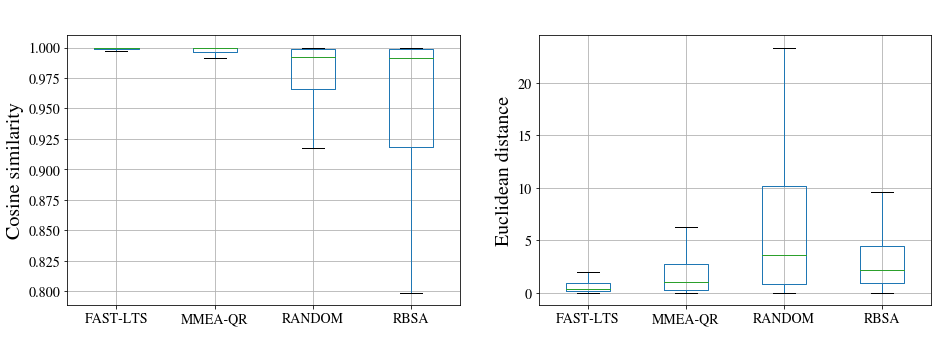
\includegraphics[width=12cm]{img/random_box}

    \caption{Cosine similarity and $L^2$ norm for multiple algorithms. Random algorithms are outperformed by the algorithms finding the weak and strong necessary conditions.}
    \label{randim:box}
\end{figure}

In Figure~\ref{randim:box} box plots describing the quality of the solution are given. The $L^2$ norm of the RBSA estimate is in average less, the cosine similarity is worse. Moreover we can clearly see that MMEA-QR and FAST-LTS provide much more reliable results (even in shorter CPU times).

There are many other possibilities for other experiments than what is provided in this chapter, especially the experiments suggested in the Section~\ref{results:combinations} for exploring domains of $h$-element subsets satisfying the weak and strong necessary conditions. These experiments are out of the scope of this work, because already provided simulations were quite exhaustive due to the lot of possible variations of the algorithms.  